\chapter{Project}

\section{Code Concept}

In extend to this article is a code base available \footnote{\url{https://www.github.com/florianwiech/incremental-machine-learning}}.
This code base includes the reimplementation of EWC and the extension of modifying the Fisher Information Matrix.
The concept documents the code structure and procedure.

The complete code consists of three files.
"main.py", "network.py" and "mnist.py".

\begin{figure}[H]
    \centering
    
\includegraphics[scale=.4]{project/concept/files}
    \caption{File structure}
    \label{fig:concept_file_structure}
\end{figure}

The "\textbf{mnist.py}" makes the mnist dataset available.
It loads the mnist database automatically, reshapes the values and data structures and splits or permutes the dataset if neccesary.
After the calculation it returns the arrays in Python standard datastructures with the extension of multi-dimensional arrays from NumPy.
\newline
"\textbf{network.py}" holds the "Network" class.
The class consists of all neccesary operations for the EWC algorithm with original and adaption.
The contructor creates a neural network with 784 input neurons, three hidden layers with each 800 neurons and the ten mnist output classes.
In addition to that it initializes all neccesary functions like loss and accuracy.
After initialization the object offers several methods for training, testing and applying EWC to the task.
Figure \ref{fig:concept_class_diagram} shows a class diagram of the Network class.

\begin{figure}[H]
    \centering
    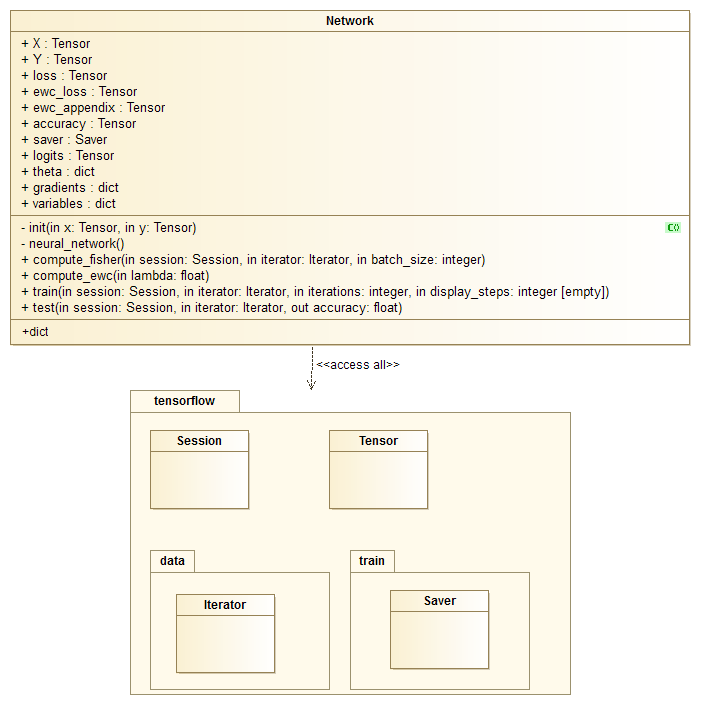
\includegraphics[scale=.6]{project/concept/class_diagram}
    \caption{Class diagram}
    \label{fig:concept_class_diagram}
\end{figure}

While execution the networks occupies multiple states.
The states distinguish if the network trains the first task or loads a previous state and retrains the network.
Figure \ref{fig:concept_state_diagram} shows the state diagram for the network:

\begin{figure}[H]
    \centering
    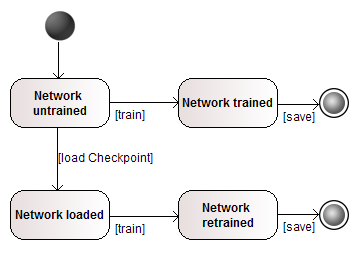
\includegraphics[scale=.8]{project/concept/state_diagram}
    \caption{State diagram}
    \label{fig:concept_state_diagram}
\end{figure}

"\textbf{main.py}" is the entrypoint of the code base.
It offers an command line tool for specification of the neccesary parameters.
\newline
The main function executes one tasks and saves their state in a checkpoint.
The task execution includes loading a checkpoint if it is not the first task or initialize a untrained network.
After that training or retraining the network and calculating the matrix if the new network should be saved.
Then perform an accuracy check on the testset and exit the script.
To train the second task the script has to be started again with different parameters.

The sequential execution is shown in a sequence diagram.
The first part (Figure \ref{fig:concept_sequence_diagram_part_1}) shows the initialization of all neccesary parameter and objects.
Part 2 (Figure \ref{fig:concept_sequence_diagram_part_2}) shows the execution of training and testing the neural network.

\begin{figure}[H]
    \centering
    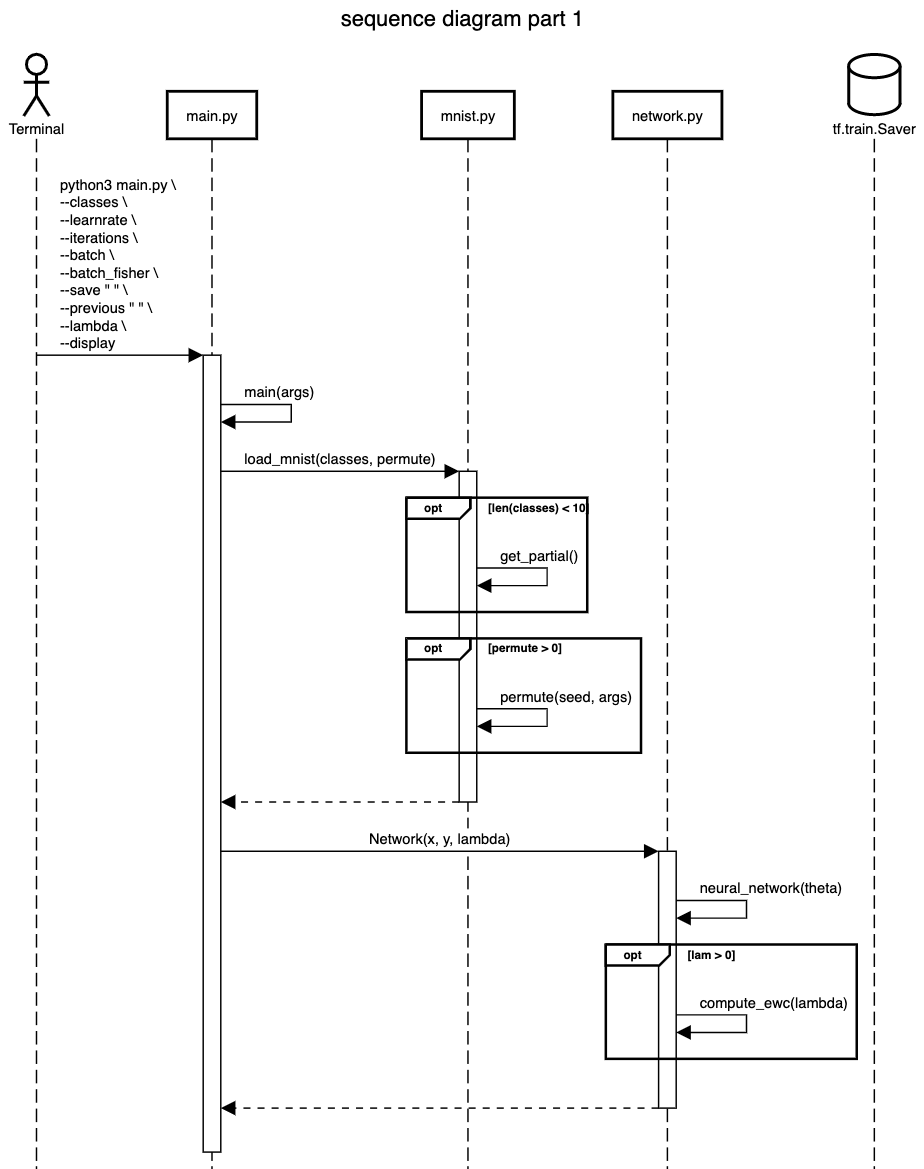
\includegraphics[width=\textwidth]{project/concept/sequence_diagram_part_1}
    \caption{Sequence diagram part 1}
    \label{fig:concept_sequence_diagram_part_1}
\end{figure}

\begin{figure}[H]
    \centering
    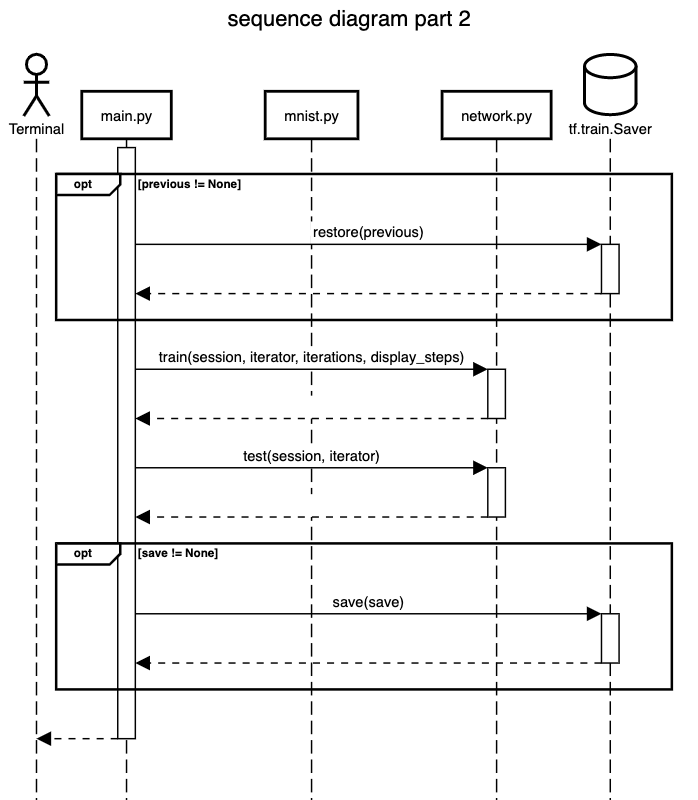
\includegraphics[width=\textwidth]{project/concept/sequence_diagram_part_2}
    \caption{Sequence diagram part 2}
    \label{fig:concept_sequence_diagram_part_2}
\end{figure}

\newpage
\section{Baseline}

Before adapting the EWC algorithm the codebase has to proof, that it delivers the results of the EWC paper.
The original EWC algorithm was tested in the constructed benchmarks described in Project Goals (Section \ref{project_goals}):

\subsection{Disjoint 9-1 Benchmark}

$T_1$ (blue, $\bigtriangleup$) trained with the classes zero to eight and reaches an accuracy of 95.72\% at the end of its training pahse.
The task was trained with a learnrate of 0.001, 2,500 iterations and an batch size of 100.
In comparison to the complete dataset (green, line), the accuracy is 86.06\%.

$T_2$ (yellow, $\bullet$) trained with the class nine further of $T_1$ uses a learnrate of 0.00001, 2,500 iterations and a batch size of 100.
The lambda value is $\frac{1}{learnrate = 0.00001} = 100,000$.
It reaches an accuracy of 97.81\%.

At the end of $T_2$ trainng phase designates $T_1$ to 84.50\% and the complete dataset 85.44\%.
The complete dataset reaches a peak of 93.43\% where $T_1$ has 94.87\% precision and $T_2$ 76.66\% precision.

Figure \ref{fig:ewc_d9-1} shows the trainings of both tasks compared to the accuracy of the complete dataset:

\begin{figure}[H]
    \centering
    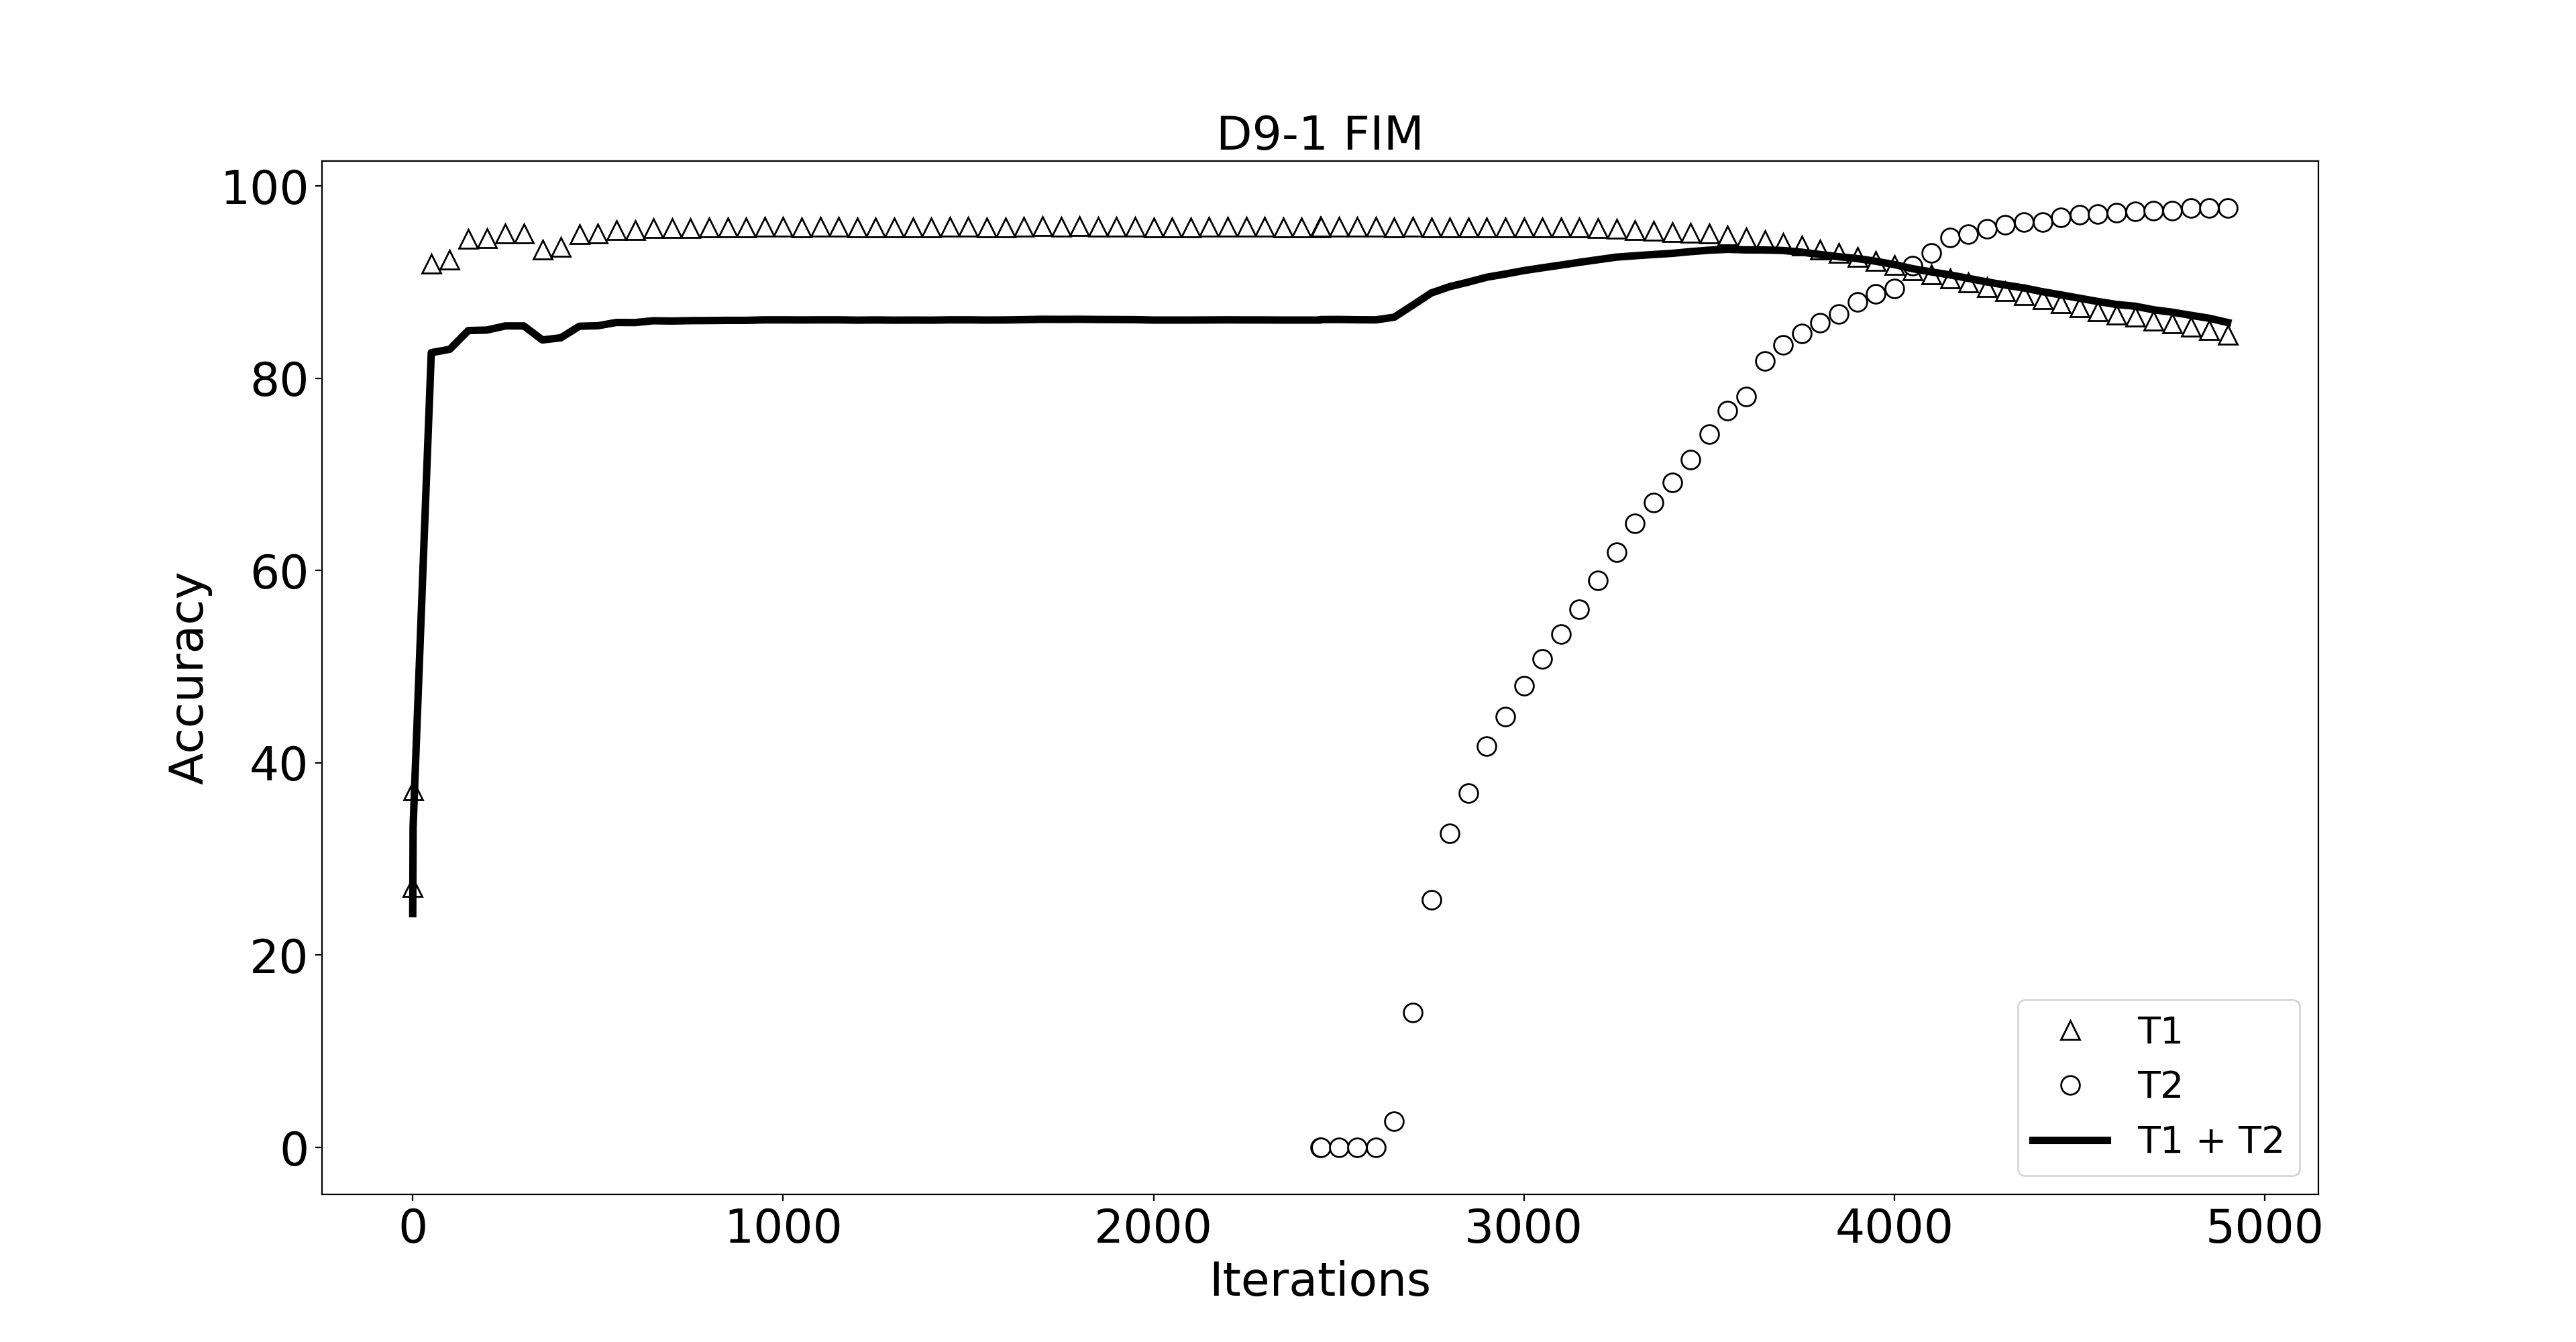
\includegraphics[width=\textwidth]{project/baseline/D91_FIM}
    \caption{EWC D9-1}
    \label{fig:ewc_d9-1}
\end{figure}

\subsection{Disjoint 5-5 Benchmark}

Figure \ref{fig:ewc_d5-5} shows training of a disjoint mnist with a five class split.

The first Task $T_1$ (blue, $\bigtriangleup$) with the classes zero to four, reached an accuracy of 98.66\% after the first training.
$T_1$ is trained with a learnrate of 0.001, 2,500 iterations and a batch size of 100.
Since there are only five of ten possible classes trained, the accuracy on the complete dataset amounts 50.70\%.

In the second training phase with task $T_2$ (yellow, $\bullet$), the classes five to nine achieve an accuracy of 82.67\%.
The learnrate of $T_2$ is 0.00001 and there were again 2,500 iterations and a batch size of 100.
Since it is an ongoing task, the EWC appendix is applied to the loss.
In this case lambda was set to $\frac{1}{learnrate = 0.00001} = 100,000$.

After the second training had $T_1$ lost 22.22\%, but still shows a quality of 76.44\%.
The performance of the complete dataset ascended from 50.70\% to 79.39\%.

\begin{figure}[H]
    \centering
    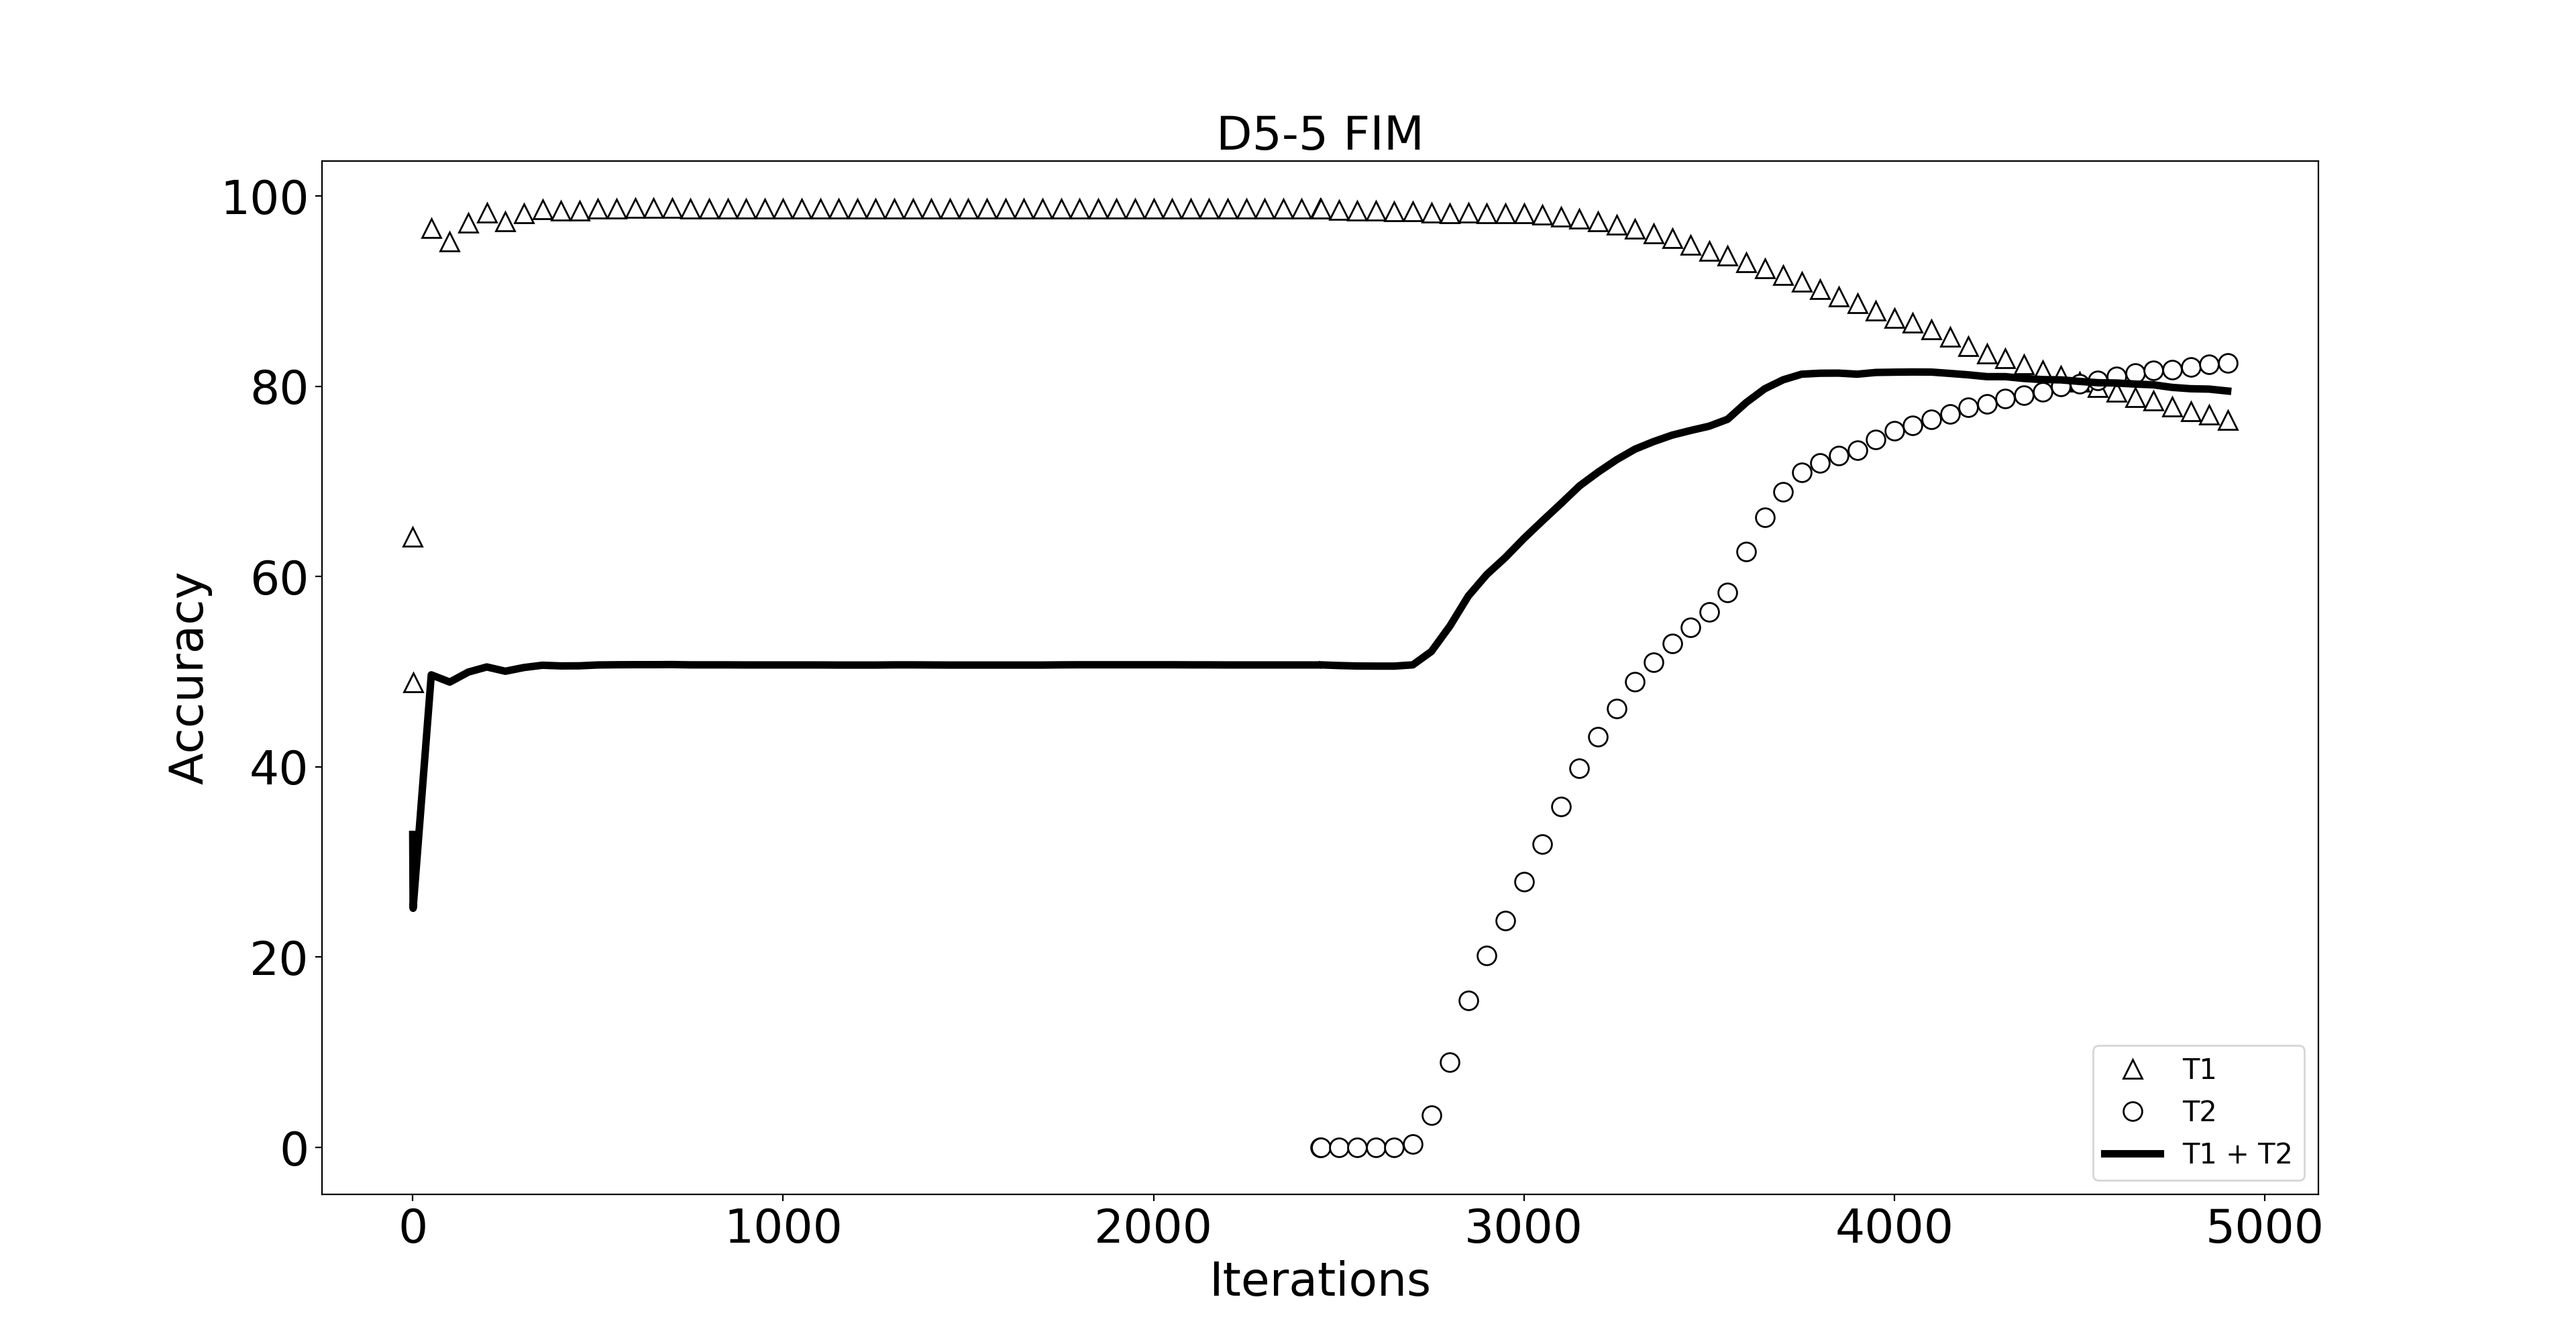
\includegraphics[width=\textwidth]{project/baseline/D55_FIM}
    \caption{EWC D5-5}
    \label{fig:ewc_d5-5}
\end{figure}

\subsection{Permuted 10-10 Benchmark}

EWC performance is shown in Figure \ref{fig:ewc_p10-10}.
$T_1$ is trained with following parameters:
all classes with a
learnrate of 0.001,
60,000 samples,
batch size of 100 in
2,500 iterations.
After the $T_1$ training, it shows an accuracy of 94.76\% which is equally to the complete dataset.
\newline
$T_2$ on the other hand learned with a rate of 0.00001 with 20,000 iterations.
The 60,000 samples were permuted with a seed of zero and split into batches with a size of 100.
The importance of the EWC loss was $\lambda = \frac{1}{0.00001} = 100,000$.
$T_2$ needed in this case a longer learnrate to be able to have an good accuracy.
It shows a performance of 91.45\% and 90.53\% on the complete dataset.
$T_1$ still performs with 94.78\%.

\begin{figure}[H]
    \centering
    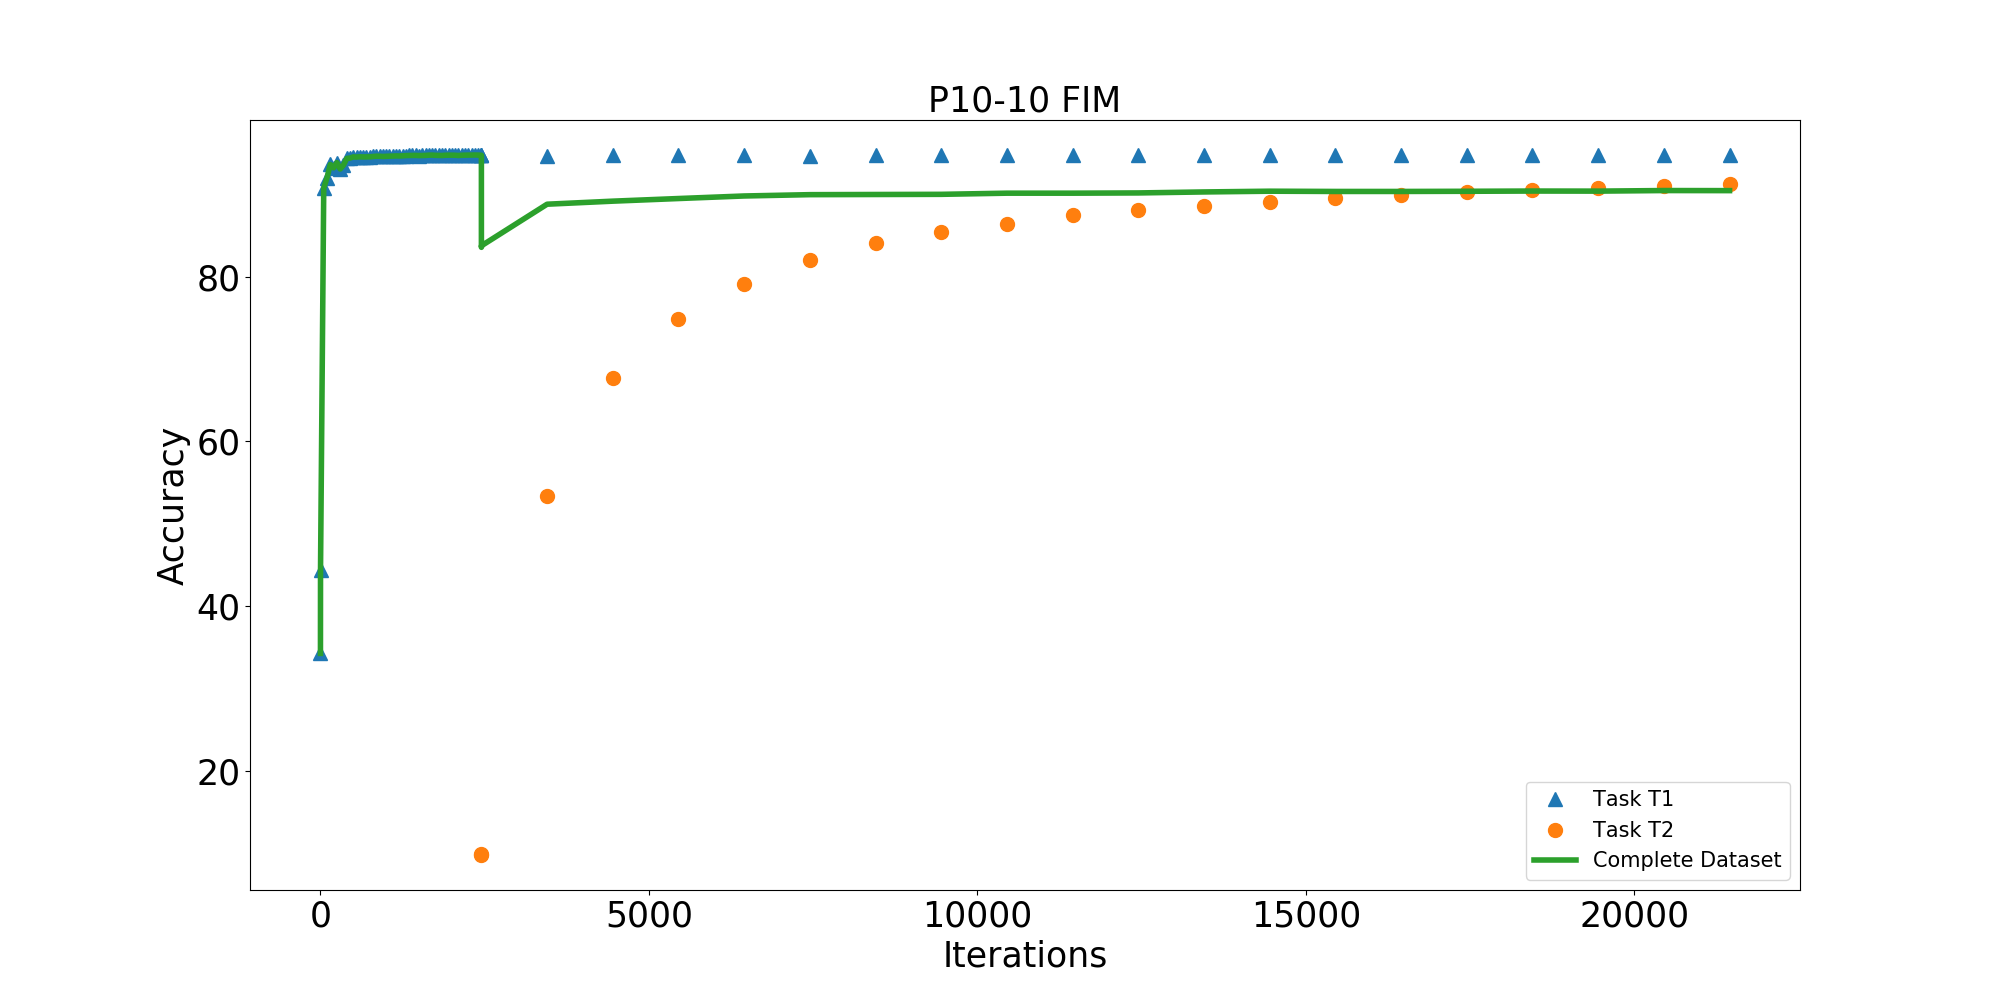
\includegraphics[width=\textwidth]{project/baseline/P10-10_FIM_IT20k}
    \caption{EWC P10-10}
    \label{fig:ewc_p10-10}
\end{figure}

\section{Critical review of EWC and improvements}
\label{project_review_improvements}

As proposed in Elastic Weight Consolidation (Section \ref{foundation_ewc}, \cite{elastic-weight-consolidation}) the authors use the diagonal of Fisher Information Matrix for the loss calculation.

$$F_{ij} = \frac{1}{N} \sum_{n}^{N} \frac{\partial \mathcal{L}}{\partial \theta_{i}} \cdot \frac{\partial \mathcal{L}}{\partial \theta_{j}}$$

$$\vec{F} \equiv diag \left(F_{ij}\right)$$

The reports \cite{better-weight-consolidation,elastic-weight-consolidation} justify that the assumption of the diagonal FIM is common practice \cite{elastic-weight-consolidation,better-weight-consolidation,incremental-moment-matching}.
It reduces the operations fom $O(N^2)$ to $O(N)$, where $N$ is the number of elements in $\theta$.
This reulsts in a lot faster calculation even in large models.
\cite{elastic-weight-consolidation,better-weight-consolidation}
Moreover, this justification receives rather promising results and holds in some cases.
\cite{elastic-weight-consolidation,incremental-moment-matching}.

The current reference implementation of EWC uses Tensorflow.
A problem with calculating the FIM in Tensorflow is that it is neccesary to get the gradients for every sample but Tensorflow does not expose them.
So this implementation built a complex workaround by hardcoding the gradients directly into the computation graph of Tensorflow.
This solutions increases the memory consumption by the batch size.
It results that the developer set the batch size for this computation to the fixed rate of 100, because the computation of a full batch would diretly run out of memory.
\cite{github_ewc_issue_one}


% -> break it down that is actualy just approximative calculation by gradients

% show our approach and why this 

The idea is it to narrow down the problem for a much easier calculation that receives the same results.
The FIM just uses the diagonal.
This means $\theta_i$ and $\theta_j$ will always be the same weight or bias matrix.
So we can summarize them to one parameter $\theta_k$.
This reults in a much simpler formula:

$$diag \left(F_{ij}\right) = F_k = \frac{1}{N} \sum_{n}^{N} \left( \frac{\partial \mathcal{L}}{\partial \theta_{k}} \right)^2$$

This simplification is still  based on a per gradient calculation.
The further idea is it to take the square of the gradient of a complete mini-batch.
Since it is common practice to create mini-batches for training a network, this modification of the matrix would solve the problem with Tensorflow and enables a much faster calculation of the matrix.
The avereged gradients of a mini-batch shouldn't have much of a difference compared to the per sample gradients.
This modification of the matrix looks like this:

$$diag \left(F_{ij}\right) = F_k = \left( \frac{1}{N} \sum_{n}^{N} \frac{\partial \mathcal{L}}{\partial \theta_{k}} \right)^2$$

An important note is that with an batch size of one, this modification would be the same as the FIM. 
The following section tests this modification on the D9-1, D5-5 and P10-10 benchmarks.

\newpage
\section{Experimental Results}

This sections show the results of EWC with the modified FIM and testing different values for the learningrate and lambda.
The network features are listed in Section \ref{foundations_deep_neural_network}.

\subsection{Disjoint 9-1}

All experiments with a disjoint nine to one test on MNIST are split in the task $T_1$ with classes zero to eight and task $T_2$ with class nine.
Task $T_1$ was trained on 54051 samples, split into batches with a size of 100.
The learnrate amounted 0.001.
This reults in a performance of 95.72\% on the $T_1$ testset and 86.06\% on the complete set.

Figure \ref{fig:exp_d9-1_bs1k} shows besides the training of $T_1$ the retraining of the network with $T_2$.
$T_2$ included 5900 samples that were split into 59 batches and tarined in 2,500 iterations.
The learnrate of the optimizer was 0.00001 and $\lambda = \frac{1}{0.00001} = 100,000$.
$T_2$ achives a performance of 97.72\%.
At the end of both trainings $T_1$ performs with 83.60\%.
The complete testset indicates an accuracy of 84.72\%, a minus of 1.34\%.

\begin{figure}[H]
    \centering
    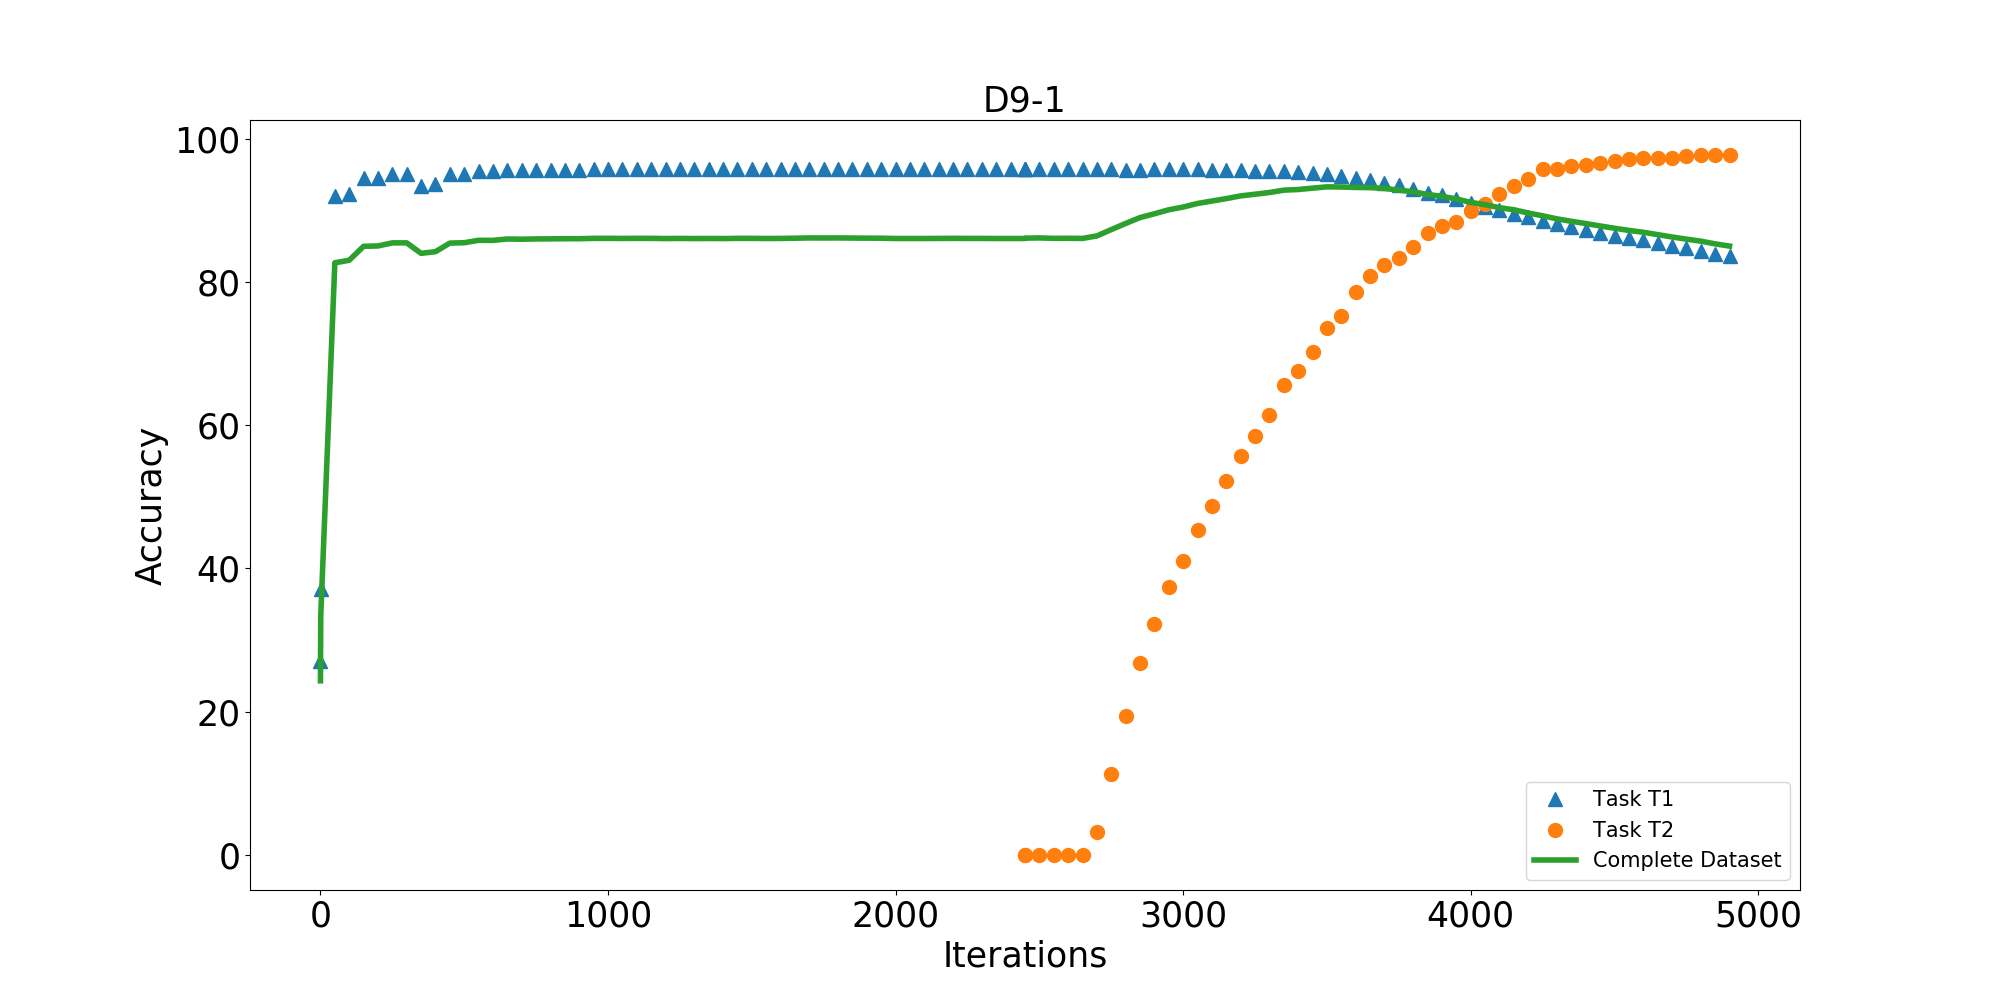
\includegraphics[width=\textwidth]{project/experiments/D91_BS1k}
    \caption{Experiment D9-1}
    \label{fig:exp_d9-1_bs1k}
\end{figure}

\newpage

Table \ref{table:exp_d9-1} tests multiple learnrates and lambda values with $T_2$ on the complete dataset.
Every parameter test was done with 2,500 iterations and a batch size of 100 and 5900 samples.
\newline
The results show that the best performance is with a learnrate of 0.00001 and a lambda value of 1,000,000. With these parameters performs $T_2$ with 87.78\%, $T_1$ has still a performance of 74.12\% and the complete dataset with 90.84\%.

\begin{table}[H]
    \centering
    \begin{tabular}{ |c|l|l|l|  }
        \hline
        \multicolumn{2}{|c|}{parameters} & \multicolumn{2}{c|}{accuracy after $T_2$ training} \\
        \hline
        learning rate & lambda & $T_2$ & complete dataset\\
        \hline
        \hline
        \multirow{6}{*}{0.001} & 1,000 & 100\% & 11.20\%\\
                            & 10,000 & 100\% & 12.78\%\\
                            & 100,000 & 100\% & 12.93\% \\
                            & 1,000,000 & 100\% & 15.92\% \\
                            & 1,010,000 & 100\% & 15.14\% \\
                            & 1,050,000 & 100\% & 14.65\% \\
        \hline
        \multirow{6}{*}{0.0001} & 1,000 & 100\% & 42.22\%\\
                                & 10,000 & 100\% & 40.47\%\\
                                & 100,000 & 100\% & 37.86\% \\
                                & 1,000,000 & 100\% & 41.99\% \\
                                & 1,010,000 & 100\% & 40.09\% \\
                                & 1,050,000 & 100\% & 40.11\% \\
        \hline
        \multirow{6}{*}{0.00001} & 1,000 & 98.91\% & 82.62\%\\
                                & 10,000 & 98.82\% & 83.48\%\\
                                & 100,000 & 97.82\% & 85.41\% \\
                                & 1,000,000 & 87.78\% & 90.84\% \\
                                & 1,010,000 & 87.69\% & 90.86\% \\
                                & 1,050,000 & 87.51\% & 90.87\% \\
        \hline
        \multirow{6}{*}{0.000001} & 1,000 & 94.27\% & 90.2\% \\
                                & 10,000 & 80.34\% & 92.81\% \\
                                & 100,000 & 3.18\% & 86.4\% \\
                                & 1,000,000 & 0.0\% & 86.17\% \\
                                & 1,010,000 & 0.0\% & 86.16\% \\
                                & 1,050,000 & 0.0\% & 86.16\% \\
        \hline
    \end{tabular}
    \caption{Experiment D9-1}
    \label{table:exp_d9-1}
\end{table}

\newpage

\subsection{Disjoint 5-5}

The disjoint 5-5 experiments a split into the classes zero to four and five to nine.
$T_1$ has 30500 samples split into 305 batches and trained with 2500 batch cycles.
The learnrate is 0.001,w hich results in a performance of 98.66\% with $T_1$ and 50.70\% on the complete dataset.

Figure \ref{fig:exp_d5-5_bs1k} show both tasks $T_1$ and $T_2$.
In this case $T_2$ was trained with 29,400 samples, a batch size of 100 and a learnrate of 0.00001.
The EWC loss was calculated with $\lambda = \frac{1}{0.00001} = 100,000$.
The result of $T_2$ training is a performance of 82.30\% on $T_2$, 76.73\% on $T_1$ and an accuracy of 79.33\% on the complete dataset.
This shows that the network achvieved an increase of 28.63\%.

\begin{figure}[H]
    \centering
    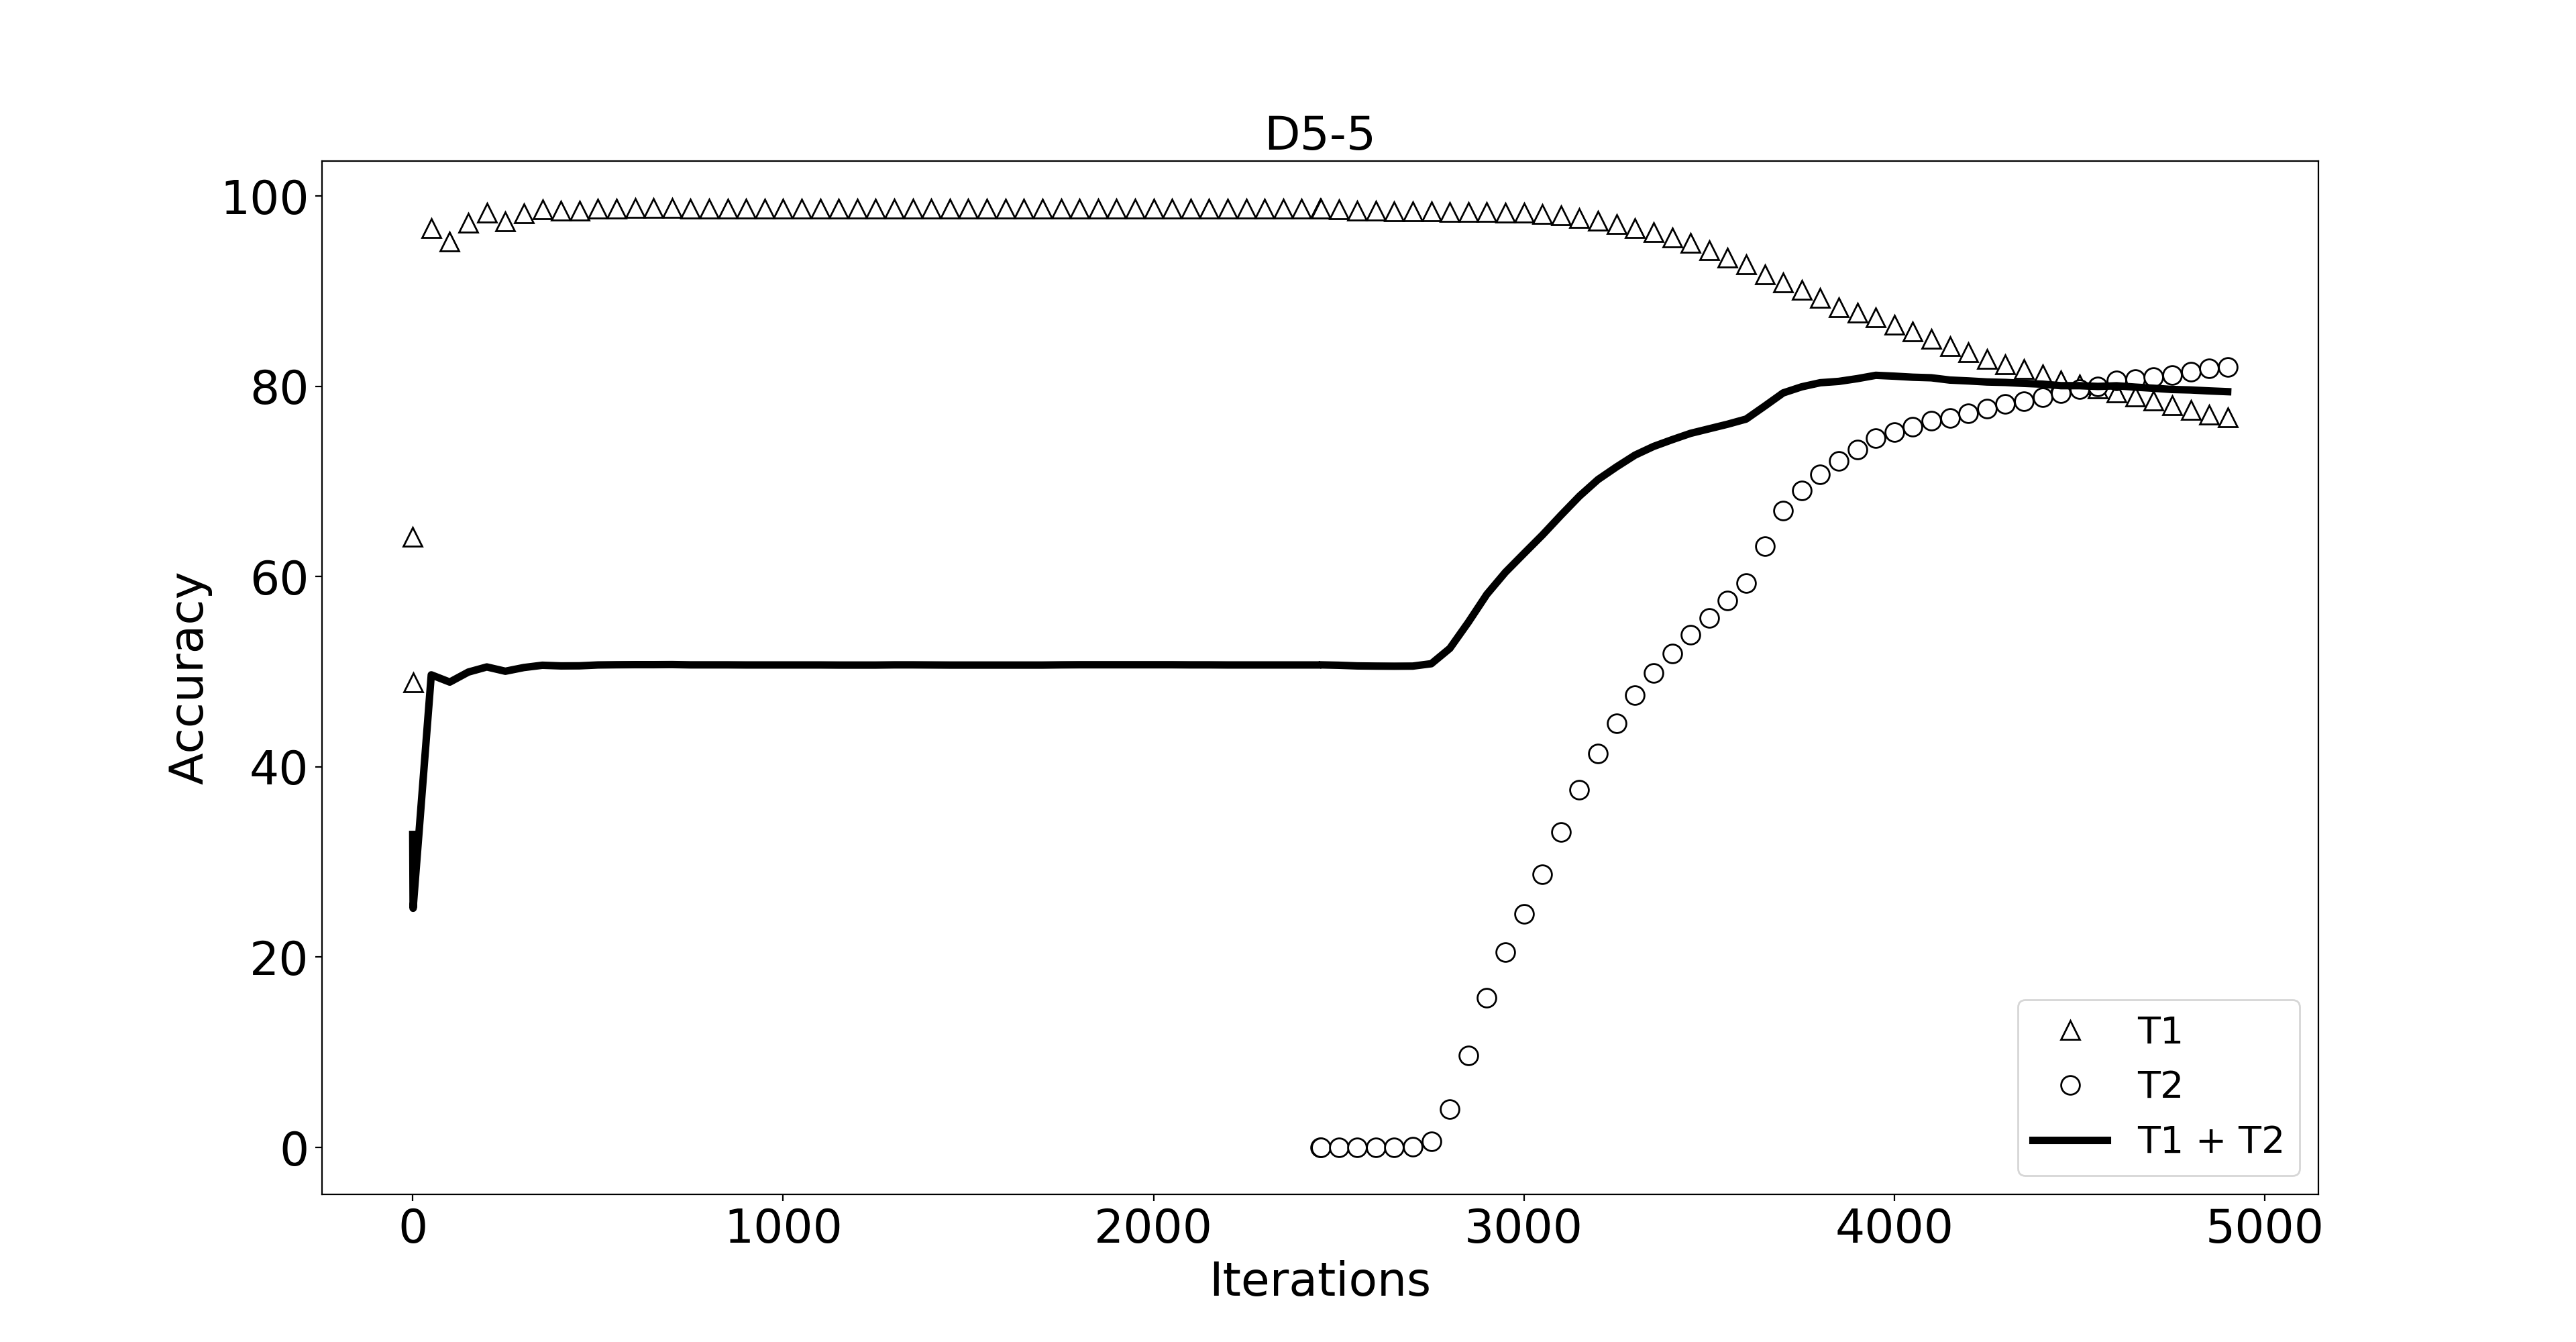
\includegraphics[width=\textwidth]{project/experiments/D55_BS1k}
    \caption{Experiment D-5}
    \label{fig:exp_d5-5_bs1k}
\end{figure}

\newpage

Table \ref{table:exp_d5-5} lists several parameter test.
These tests were built on the same parameters for $T_2$ exept the learnrate and lambda was varied.
The best result is with the learnrate of 0.00001 and a lambda value of 1,000.
It shows that the complete set has an accuracy of 81.87\%, $T_2$ of 93.64\% and $T_1$ of 71.16\%.

\begin{table}[H]
    \centering
    \begin{tabular}{ |c|l|l|l|  }
        \hline
        \multicolumn{2}{|c|}{parameters} & \multicolumn{2}{c|}{accuracy after $T_2$ training} \\
        \hline
        learning rate & lambda & $T_2$ & complete dataset\\
        \hline
        \hline
        \multirow{6}{*}{0.001} & 1,000 & 97.87\% & 48.94\%\\
                            & 10,000 & 98.13\% & 49.84\%\\
                            & 100,000 & 97.94\% & 51.04\% \\
                            & 1,000,000 & 97.5\% & 51.72\% \\
                            & 1,010,000 & 97.27\% & 51.99\% \\
                            & 1,050,000 & 97.52\% & 52.75\% \\
        \hline
        \multirow{6}{*}{0.0001} & 1,000 & 97.05\% & 63.24\%\\
                                & 10,000 & 96.65\% & 63.49\%\\
                                & 100,000 & 96.19\% & 61.74\% \\
                                & 1,000,000 & 95.65\% & 63.14\% \\
                                & 1,010,000 & 95.74\% & 63.06\% \\
                                & 1,050,000 & 95.59\% & 63.03\% \\
        \hline
        \multirow{6}{*}{0.00001} & 1,000 & 93.64\% & 81.87\%\\
                                & 10,000 & 90.45\% & 83.49\%\\
                                & 100,000 & 82.38\% & 79.86\% \\
                                & 1,000,000 & 67.84\% & 72.68\% \\
                                & 1,010,000 & 67.79\% & 72.64\% \\
                                & 1,050,000 & 67.2\% & 72.42\% \\
        \hline
        \multirow{6}{*}{0.000001} & 1,000 & 28.1\% & 63.55\% \\
                                & 10,000 & 18.9\% & 59.39\% \\
                                & 100,000 & 0.02\% & 50.6\% \\
                                & 1,000,000 & 0.0\% & 50.71\% \\
                                & 1,010,000 & 0.0\% & 50.71\% \\
                                & 1,050,000 & 0.0\% & 50.71\% \\
        \hline
    \end{tabular}
    \caption{Experiment D5-5}
    \label{table:exp_d5-5}
\end{table}

\newpage

\subsection{Permuted 10-10}

This experiment type performs in $T_1$ a training on the complete dataset and in $T_2$ on a permuted dataset with the random seed of zero.
\newline
$T_1$ properties are: 60,000 samples into 60 batches with a size of 100, a learnrate of 0.001 and 2,500 iterations.
This results in an accuracy of 94.76\%.
The matrix calculation fot the EWC loss used a batch size of 1,000.
\newline
This experiment was as well as the baseline trained with 20,000 iterations on $T_2$.
The change of the learning rate to 0.00001 and $\lambda = \frac{1}{0.00001} = 100,000$, $T_2$ achives a performance of 91.53\%.
The complete dataset shows an accuracy of 90.45\% and $T_1$ of still 94.76\%.

\begin{figure}[H]
    \centering
    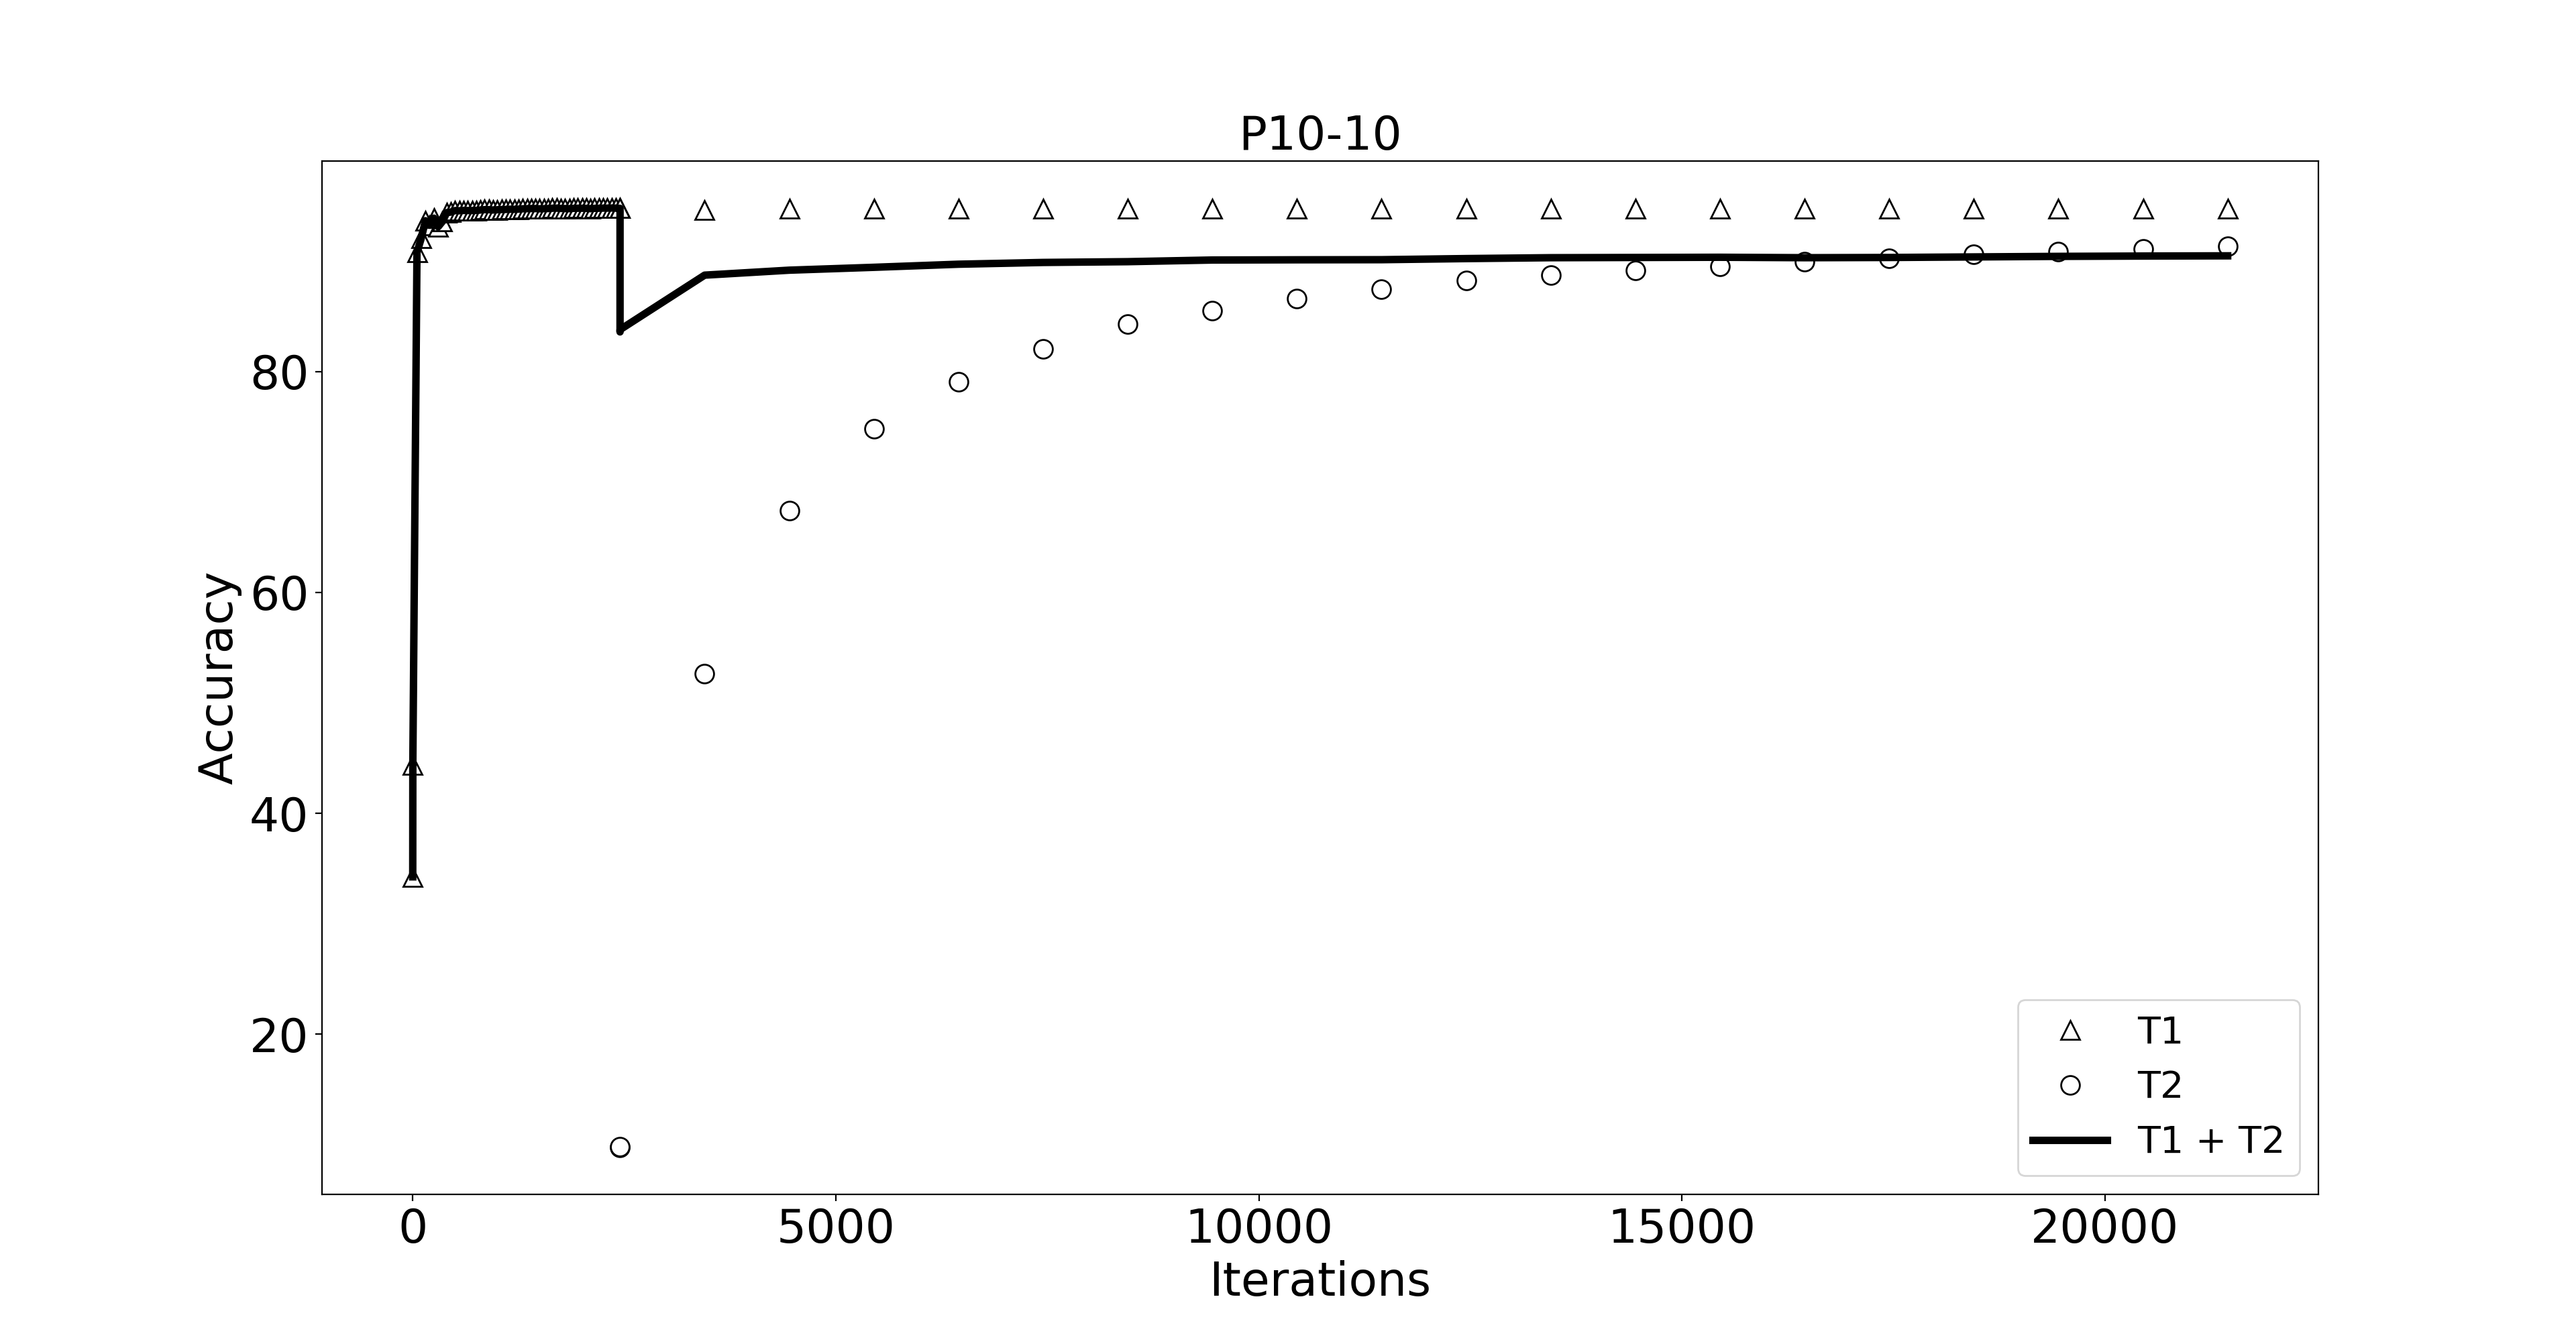
\includegraphics[width=\textwidth]{project/experiments/P10-10_BS1k_IT20k}
    \caption{P10-10}
    \label{fig:exp_p10-10}
\end{figure}

\newpage

Table \ref{table:exp_d10-10} shows the results of several experiments with the learning rate and lambda of $T_2$.
The table shows that there are many good outcomes.
The best outcomes are with the same learnrate as $T_1$ and rather small lambda value.

\begin{table}[H]
    \centering
    \begin{tabular}{ |c|l|l|l|  }
        \hline
        \multicolumn{2}{|c|}{parameters} & \multicolumn{2}{c|}{accuracy} \\
        \hline
        learning rate & lambda & $T_2$ & complete dataset\\
        \hline
        \hline
        \multirow{6}{*}{0.001} & 1,000 & 97.09\% & 93.72\%\\
                            & 10,000 & 97.66\% & 94.20\%\\
                            & 100,000 & 97.2\% & 93.05\% \\
                            & 1,000,000 & 97.3\% & 93.26\% \\
                            & 1,010,000 & 97.25\% & 92.46\% \\
                            & 1,050,000 & 96.84\% & 92.29\% \\
        \hline
        \multirow{6}{*}{0.0001} & 1,000 & 96.87\% & 91.41\%\\
                                & 10,000 & 96.51\% & 90.93\%\\
                                & 100,000 & 96.48\% & 91.45\% \\
                                & 1,000,000 & 96.45\% & 91.47\% \\
                                & 1,010,000 & 96.56\% & 91.43\% \\
                                & 1,050,000 & 96.45\% & 91.38\% \\
        \hline
        \multirow{6}{*}{0.00001} & 1,000 & 94.67\% & 90.98\%\\
                                & 10,000 & 93.04\% & 90.67\%\\
                                & 100,000 & 91.53\% & 90.46\% \\
                                & 1,000,000 & 90.29\% & 90.66\% \\
                                & 1,010,000 & 90.28\% & 90.65\% \\
                                & 1,050,000 & 90.23\% & 90.66\% \\
        \hline
        \multirow{6}{*}{0.000001} & 1,000 & 87.84\% & 89.75\% \\
                                & 10,000 & 80.58\% & 89.67\% \\
                                & 100,000 & 68.64\% & 89.17\% \\
                                & 1,000,000 & 56.66\% & 88.64\% \\
                                & 1,010,000 & 56.62\% & 88.63\% \\
                                & 1,050,000 & 56.51\% & 88.62\% \\
        \hline
    \end{tabular}
    \caption{Experiment P10-10}
    \label{table:exp_d10-10}
\end{table}
